\documentclass[]{report}
\renewcommand\thesection{\arabic{section}}%for page numbering in arabics
\usepackage{graphicx,tabularx}%for figures and tables
\usepackage[utf8]{inputenc} %allows special characters such as ä, ö, ỳ
\usepackage[english]{babel}  %set the language to English
\usepackage[margin=1.5in]{geometry} %change page margins 
\usepackage{sectsty}%section headers
\allsectionsfont{\sffamily\large}
\subsectionfont{\sffamily\normalsize}
\linespread{1.2}% line distance
\usepackage{lipsum}% http://ctan.org/pkg/lipsum
\usepackage{caption}%use for captions on tables
%use this exact command. The style and bibliographystyle has to be authoryear (Havard). The sorting is nyt: name, year, title so that the bibliography is sorted alphabetically. firstinits=true shortens the names: Albert Einstein -> A. Einstein
\setcounter{secnumdepth}{3}
\setcounter{tocdepth}{3}
\usepackage[backend=bibtex,style=authoryear,bibstyle=authoryear,sorting=nyt,firstinits=true]{biblatex}
\setlength\parindent{0pt}%include this so that your paragraphs don't indent automatically
\addbibresource{report.bib} %this attaches your bib-file, your bibliography (must be in the same folder)
\usepackage[compact]{titlesec}%include title formatting package
\usepackage[section]{placeins}
\usepackage{placeins}
\titleformat*{\subsubsection}{\normalsize\bfseries}


% Title Page
\title{Top Text}
\author{Tom Jacobs and James Boogaard}
\date{December 15th 2022 \\Module: SEAR \\Venlo, Limburg, Netherlands}


\begin{document}
	
	\maketitle
	
	\begin{abstract}
		Following the explosion of artificial intelligence during the year of 2022, there now are many text-to-image generation applications out there. This is great for the field of artificial intelligence as a whole, however it has made knowing which application is best quite hard for artists who are new to text-to-image generation. This paper looks at four of the most popular generators, with the aim to find out which one is the best for an inexperienced artist.
		
		\pagenumbering{roman}
		
	\end{abstract}
	
	\tableofcontents
	\setcounter{page}{3}
	\listoffigures %UNCOMMENT IF YOU HAVE FIGURES
	%\listoftables %UNCOMMENT IF YOU HAVE TABLES
	\pagebreak
	
	\pagenumbering{arabic}	
	
	\section{Introduction}
	
	\subsection{Context and background}
During the year of 2022 there has been a massive increase in the popularity and use of text-to-image generators, an artificial intelligence technique that translates human text into a computer-generated image. You will likely have heard of at least one of these if you frequent the internet. This explosion in popularity has led to many different text-to-image applications being made, which on the one hand has given many more options to artists(people who use a text-to-image generator to create and refine an image), but it has also made the landscape more difficult to navigate because of its abundance of choice. This paper makes an effort to try and alleviate this problem by picking four of the most used text-to-image generators and comparing them based on their accuracy and process. This allows us to help people gain some perspective on which text-to-image generator is best for their needs.

A research paper was published on the nineteenth of February 2020 called: "A survey and taxonomy of adversarial neural networks for text-to-image synthesis" that makes use of surveys to compare models for text-to-image generations. This paper aimed to show which text-to-image technique yielded the most realistic results in a wide variety of categories. One issue with this paper was that is was written before the explosion of consumer text-to-image generators happened, which is why we will instead focus on modern consumer-grade generators which are available today.

	\subsection{Problem and hypothesis}
Our goal during the course of this research paper is to find out what the best text-to-image generator is out of the four we chose, in the case of an artist who is not experienced in the world of text-to-image generation. Our hope is that artists who are new to text-to-image generation will be able to make an educated decision on which generator is best for them on the basis of this paper.

Another question we take a look at is what makes an application good for an inexperienced artist. In answering this question we will consider: the tools available to an artist, the difficulty in using these tools, the accuracy in generating images, the learning curve of an application and the speed with which the application can generate images. With these points of consideration it should be possible to score each application on their ease of use, and on their future potential if the artist were to stick with that application.

The text-to-image generators we will be testing during the course of this paper are: Stable diffusion, Midjourney, DallE and Dream by Wombo. We came to these models after looking at several applications in google trends. This gave us a good idea of what the landscape looked like, and which applications artists would be likely to choose. You may notice below in Figure 1 that Dream by Wombo is not that popular anymore, however it was one of the first openly accessible text-to-image applications out there.

\begin{figure}[!h]
	\centering
	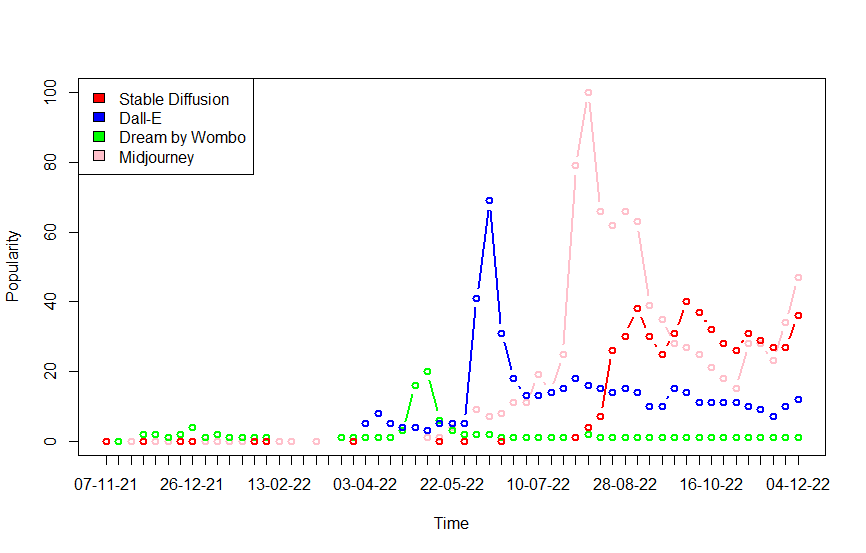
\includegraphics[width=1\linewidth]{TrendsPlotWithLegend}
	\caption{Results from Google Trends showing the popularity of different text-to-image applications}
	\label{fig:TrendsPlotWithLegend}
\end{figure}

\pagebreak

We expect the best text-to-image generator out of the four we chose to be stable diffusion. This is due to the fact that stable diffusion offers its users more tools and techniques like inpainting (allows you to regenerate a specific area of an image without regenerating the whole image), this allows the user more freedom to fine-tune their result. Given enough time this will yield a more accurate result.
	
\pagebreak
	
	\section{Methods}
	
	\subsection{Data collection}
	Our goal during the course of this research paper is to find out what the best text to image generator is, out of the four we chose, for artists who are inexperienced in AI art generation.
	
	In order to find out which is the best one, we will first look at the accuracy with which the generator can create images. We will score the accuracy with an API developed by DeepAI which can calculate image similarity.
	
	
	\subsubsection{Generating images}
	
	We have chosen an image that we find sufficiently covers all the challenging parts of recreating an image using ai art generation such as reflections and complex composition(see figure 2 below).
	Subject 1 has experience with Midjourney and Subject 2 has experience with Stable diffusion and neither of them have any experience in the other applications. Both Subject 1 and Subject 2 then use each of the four text-to-image generation applications to try and recreate that image within a given time frame (15 minutes per application). After each iteration we take the generated image and add it to a list of the iterations for that application. 
	
	\begin{figure}[!h]
		\centering
		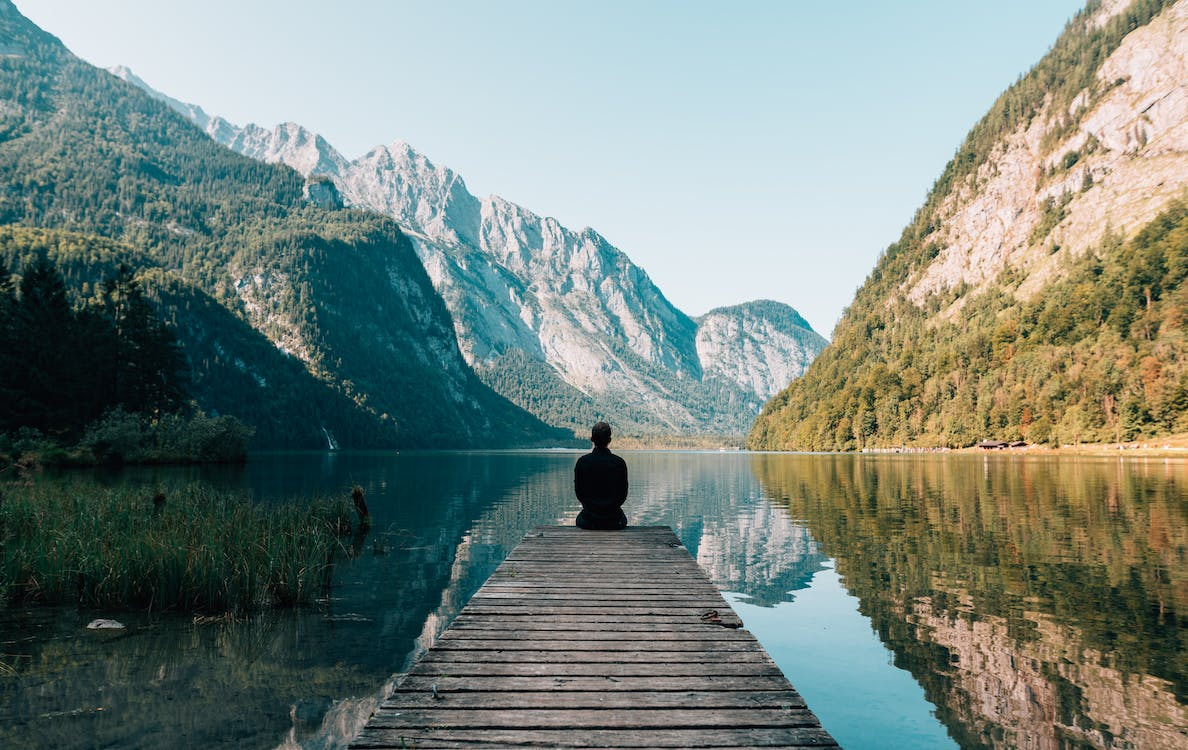
\includegraphics[width=1\linewidth]{OG}
		\caption{}
		\label{fig:og}
	\end{figure}
	
	\subsubsection{Scoring generated images}
	With those sets of data, we then plug the images (each iteration) into the image similarity checking API, developed by DeepAI, that can give you a numerical value for how close one image is to another. This way we can see how close each iteration is to the image we are trying to recreate. The amount of iterations each application is able to create then gives us insight into how fast the application is and how many iterations you have to do to achieve a certain result. We also gain an idea of how easy to use each application is through this process.
	
	In order to compare the image generation applications effectively we observe a multitude of factors that will indicate the strengths and weaknesses of that application. These factors are: The amount of iterations each participant can generate while trying to create the image within the 15 minute time limit, how close each iteration is to the image we are trying to replicate using the ai image comparing API's unit of measurement (the unit is called distance. The closer to zero the distance is, the closer the images are together. Zero means that the two images that are being compared are exactly the same), how easily we were able to access the application and its functionality, how much functionality each application offers and their effects on the final results of our experiment.
	
	
	\subsection{Visualizing data}
	
	Once the data is gathered, we can create graphs to compare the applications more easily. 
	
	In these graphs the x value is the array of different applications that we use and the y value is the result of that (the distance) for each iteration on the road to trying to recreate an image using these applications. The intervening variable in this case would be the amount of experience using these applications.
	
	We also want to check each applications average result across both Subject 1 and Subject 2 in order to compare how close each iteration gets to the original image on average. This will show us if there are any large differences between the applications as a whole. If there is this will play a role in choosing which is the best application.
	
	The last set of important data we want to visually represent is the min and max of each application and how far spread the results of each application are in order to see how reliable each application is. 
	
	
	
	\pagebreak
	
	\section{Results}

	
    
	\begin{figure}[!!htbp]
		\centering
		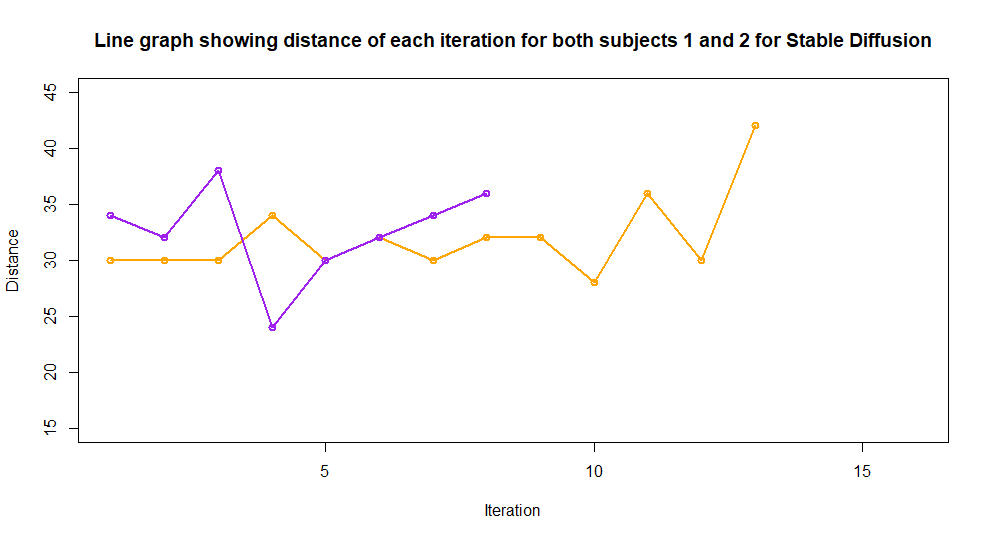
\includegraphics[width=1\linewidth]{LineGraphStableDiff}
		\caption{}
		\label{fig:linegraphstablediff}
	\end{figure}

\begin{figure}[!htbp]
	\centering
	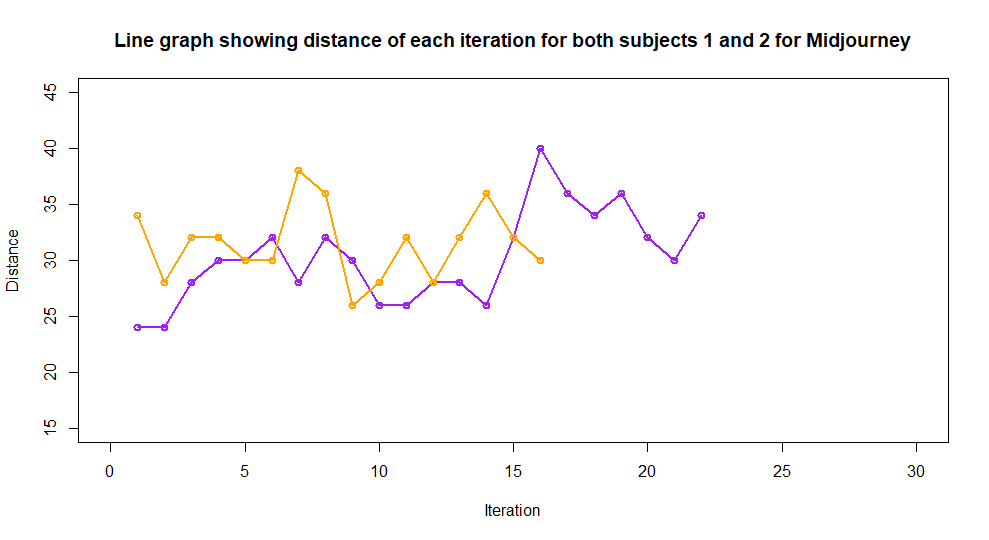
\includegraphics[width=1\linewidth]{LineGraphMidJ}
	\caption{}
	\label{fig:linegraphmidj}
\end{figure}

\subsection{Figure 3 and 4}

What is interesting in both figure one and two is that the discrepancy between the two subjects in both applications is larger than that of any of the other applications we tested. This is seen with Subject two having nearly double the amount of iterations when compared to Subject one in figure 3 and then Subject 1 having more iterations than Subject two in figure 4. Another point of interest is that the application in figure one has as a small amount of iterations when compared to the other applications. 
\begin{figure}[!htbp]
	\centering
	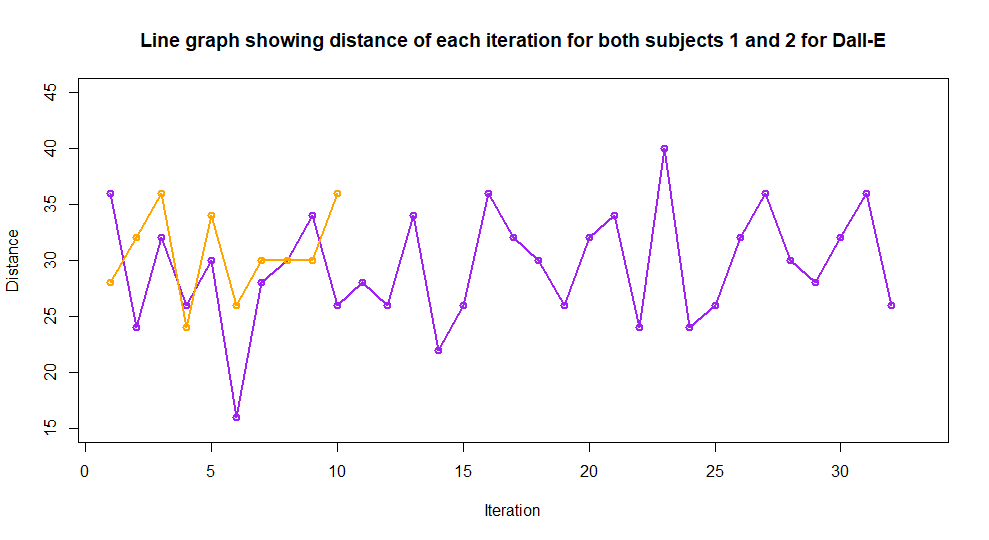
\includegraphics[width=1\linewidth]{LineGraphDall-E}
	\caption{}
	\label{fig:linegraphdall-e}
\end{figure}

\begin{figure}[!htbp]
	\centering
	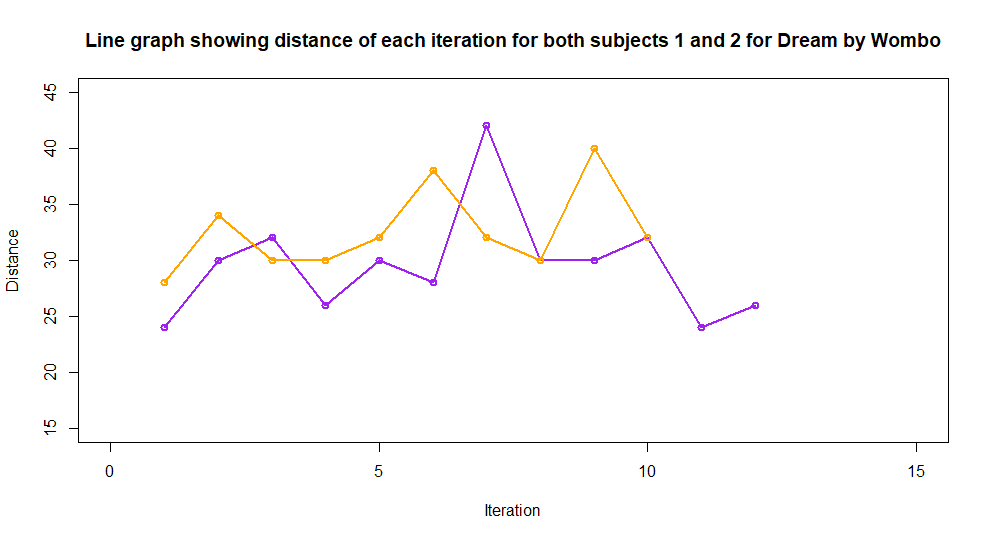
\includegraphics[width=1\linewidth]{LineGraphDBW}
	\caption{}
	\label{fig:linegraphdbw}
\end{figure}

\pagebreak
\subsection{Figure 5 and 6}

In figure 5 we see it has the most iterations out of any of the other applications. When comparing the amount of iterations that each subject has in both figure on and figure two, these two applications are very close.(-This can be attributed to the fact that the amount of experience with these graphs is very similar for both subjects-)



\begin{figure}[!htbp]
	\centering
	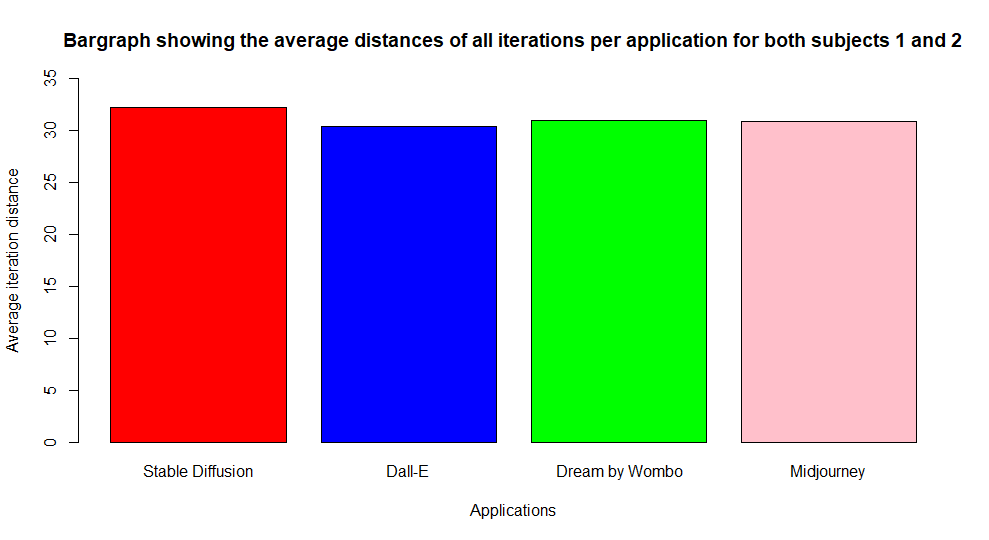
\includegraphics[width=1\linewidth]{Bargraph}
	\caption{}
	\label{fig:bargraph}
\end{figure}
\pagebreak
\subsection{Figure 7}
Figure 5 shows that the average distances of all the applications from broth subjects one and two are very close.(this is due to the random nature of t-i-g and shows that a good application is more judged by the functionality it offers rather than its algorithm when it comes to new comers). When comparing the applications Dall-E has the least average distance and stable diffusion has the most average distance but again only by a slight margin. 
	
	\begin{figure}[!htbp]
		\centering
		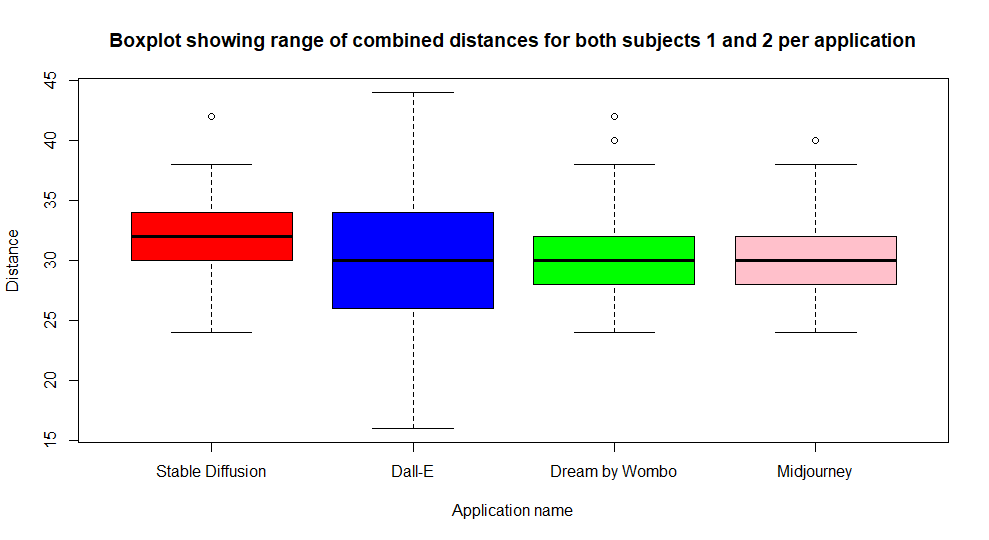
\includegraphics[width=1\linewidth]{boxplotWithAllData}
		\caption{}
		\label{fig:boxplotwithalldata}
	\end{figure}
\pagebreak
\subsection{Figure 8}
	
	In Figure 8 there are two important points of interest. Firstly is that Dall-E has a massive range between the minimum and maximum distances when compared to the other applications as well as having the largest space between q2 and q3. This means the spread of the distances is also the largest out of any of the other applications. Second is that Stable Diffusion has the largest median distance. Mention something about the outliers.
	
	
	\pagebreak
	\section{Discussion}
	
	\subsection{Interpretation}
	
	During the course of this research we were able to prove the legitimacy of our secondary research question. This was done by a analysing figures two through to six. The applications shown in figure two and three are applications that both subjects have experience in(Subject 1 has experience with Midjouney and Subject 2 has experience with Stable diffusion). What makes figure two and three important is that both the graphs show the difference that having experience in an application makes, and that difference is only in the amount of iterations the user is able to generate. 
	

	
	In figure three and four we then see two applications that neither Subject 1 nor Subject 2 have any prior experience in. using comparative analysis we can then compare both the graphs that the users have experience in (being figure two and three ) and the graphs that the subjects don't have experience in ( being figure four and five ) and we can see more clearly that when both subjects have the same amount of experience with an applications the amount of iterations the subjects are able to generate is noticeably closer together. 
	

	
	When we take a look at figure six we can see that even though even though it is the combinations of the averages of all iterations across both Subject 1 and 2 per application, the differences between the bars in very small. This can be attributed to the nature of text-to-image generation being that of a random series of attempt until the user reaches a point where they are happy with the picture. This is further proven when you look at any of the patterns for figures 2 through 5 and how the distance for each iterations follows no solid pattern but rather jumps around sometimes even ending up further away from the original image than some of the earlier iterations.
	
	
	\subsection{Secondary research question justification}
	
	In order to answer the secondary research question we looked at how different aspects of the applications affected the resulting images that were generated and came to the conclusion that the amount of functionality does not play a role in the quality of an of generated images with inexperienced users which makes sense as they may struggle to use said functionality(! add section on ease of use Stable diffusion we looking at you -This however only applies for artists who are already experienced, because it can take quite some practice to get used to all the tools that are available in stable diffusion. We expect inexperienced artists to struggle finding the right settings because of the amount of freedom they get. In the case of a completely inexperienced artist, they might find Dall-E or Midjourney easier to use because they can create photo-realistic results without having to fine tune any settings apart from the prompt.-). This can be seen when you take into consideration that stable diffusion has the most functionality but it has the worst average iteration quality across both users. 
	
	
	With all this information we can now say that an application's value to an inexperienced user is not about how good the AI generations technique is because AI text-to-image generation is very random and relies a lot on luck even for users that are experienced with applications. What we do know is that if all the applications rely on luck to some degree it is then better if the application is able to give many iterations because the more attempts you are able to make the faster you are more likely to get the result you are looking for. 
	
	\subsection{Answering primary research question}
	
	Our primary research question can then be answered now that we know what makes a good ai text-to-image application and that is how fast the application is able to generate iterations. With this in mind we can then say that Dall-E has the most iterations. It also offers a very streamline user experience and is easy to access and intuitive to use.
	
	\subsection{Further research}
	
	The ways in which our research can be carried out in an improved manner are to firstly use a bigger sample size in order make the results of the research more convincing. This can be done by using more text-to-image applications and trying to recreate more than just one picture. 
	
	Secondly you can use many different ways to compare images rather than just one in order to make the results more accurate. This can be done with surveys where you ask people which image is closer to a humans perspective or by using not just one application for image comparison.
	
\end{document}


\printbibliography[title=References]

\end{document}          
       
